\subsection{}
Un émetteur (E) d’une onde sonore et deux récepteurs (R1 et R2) voyagent à vitesse $v$, plus petite que la vitesse du son, dans les directions indiquées (R1 et E se déplacent vers la droite, R2 se déplace vers la gauche). Lequel des deux récepteurs recevra le son avec la plus grande fréquence ?
\begin{figure}[h]
    \centering
    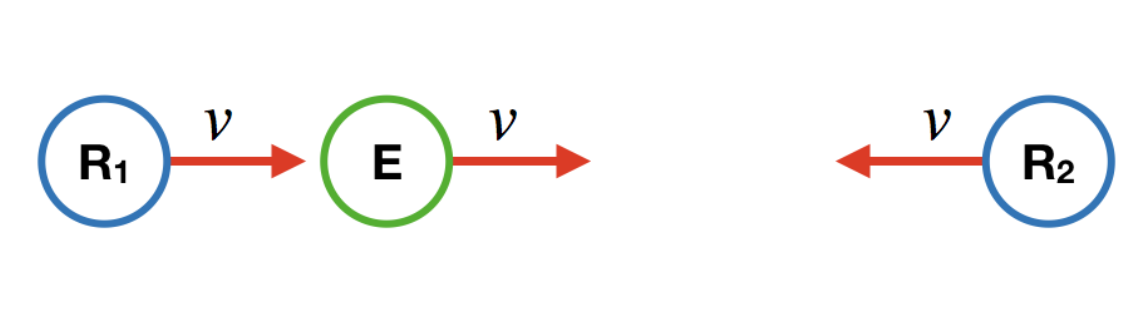
\includegraphics[width=0.9\linewidth]{Figures/1emetteur2recepteur.png}
\end{figure}
\begin{enumerate}[label=\Alph*)]
    \item Le récepteur R1.
    \item Le récepteur R2.
    \item Les deux récepteurs reçoivent un son avec une fréquence identique.
    \item Impossible de le savoir sans connaître la valeur de la vitesse $v$.
\end{enumerate}

\noindent\textbf{Justification :} \hrulefill \\[2.5ex]
\rule{\linewidth}{0.4pt} \\[2.5ex]
\rule{\linewidth}{0.4pt}
\vfill